\section{Ảnh hưởng của các cách tiền xử lý}
\label{sec:6_2}
Giữ nguyên Logistic Regression $C=1$ và thay từng thành phần riêng lẻ. Kết quả mean/SD được tính trên cùng ba fold:
\begin{table}[htbp]
\centering\scriptsize
\caption{Đối chiếu các lựa chọn tiền xử lý với Logistic Regression C=1}\label{tab:cv-preprocessing}
\begin{tabular}{lrrrr}
\toprule
Cấu hình & F1 CV & SD & Precision & Recall \\
\midrule
lr\_c1 & 0,6557 & 0,0078 & 0,7315 & 0,5943 \\
lr\_missing\_constant & 0,6586 & 0,0062 & 0,7350 & 0,5967 \\
lr\_ordinal & 0,5570 & 0,0067 & 0,7139 & 0,4567 \\
lr\_minmax01 & 0,6475 & 0,0059 & 0,7276 & 0,5833 \\
lr\_minmax11 & 0,6536 & 0,0065 & 0,7317 & 0,5906 \\
\bottomrule
\end{tabular}
\end{table}
\begin{figure}[htbp]
\centering
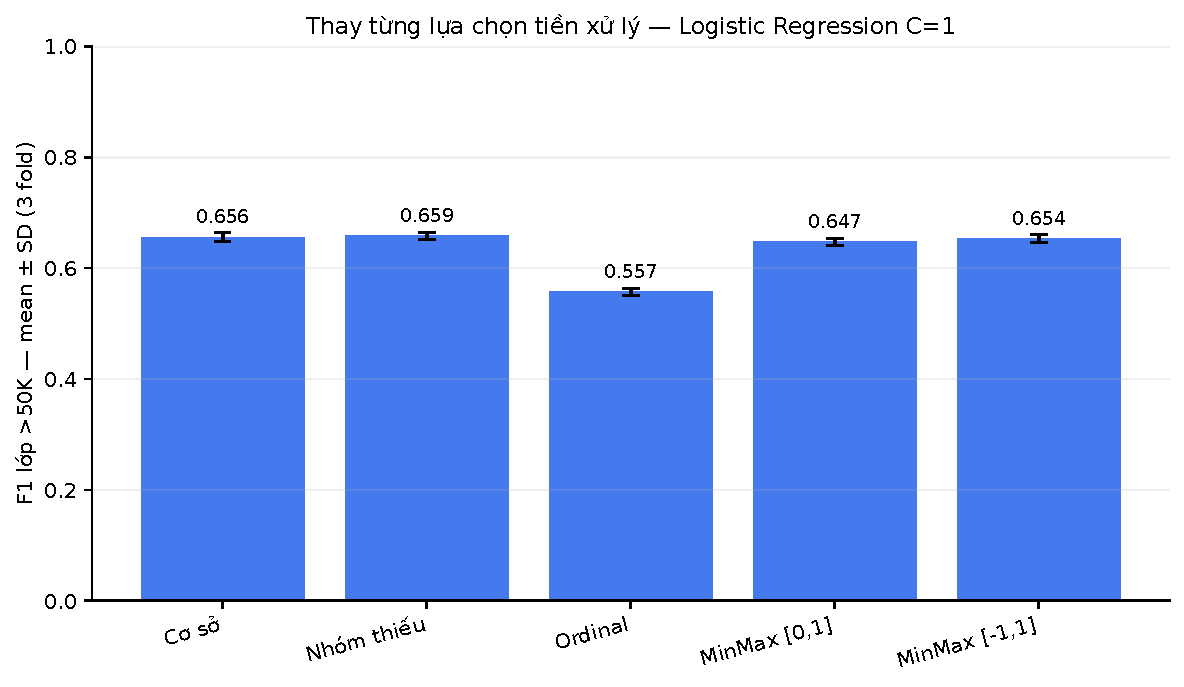
\includegraphics[width=.95\textwidth]{Images/chapter_6/6_2/cv_preprocessing.pdf}
\caption{Ảnh hưởng của các lựa chọn tiền xử lý trong thí nghiệm kiểm soát}
\label{fig:cv-preprocessing}
\end{figure}
Trong nhóm này, cấu hình có F1 trung bình cao nhất là \texttt{lr\_missing\_constant}, đạt 0,6586. Kết quả chỉ phản ánh các lựa chọn đã khảo sát. Ordinal tạo thứ tự số cho thuộc tính vốn có thể không có thứ tự tự nhiên; thay đổi này ảnh hưởng trực tiếp đến biên tuyến tính. Tác động của scaling còn phụ thuộc regularization đang giữ cố định, nên không kết luận một scaler luôn tốt hơn trên mọi mô hình.

% BEGIN REVIEW ANALYSIS
So với mốc one-hot, mode và StandardScaler, nhóm thiếu riêng làm F1 tăng 0,29 điểm phần trăm; ordinal làm F1 thay đổi -9,87 điểm phần trăm. Hai khoảng MinMax [0,1] và [-1,1] thay đổi lần lượt -0,82 và -0,21 điểm phần trăm. Các hiệu số là chênh lệch F1 trung bình nhân 100, không phải mức tăng tương đối. Mức tăng nhỏ của cách biểu diễn thiếu riêng chưa đủ để kết luận có khác biệt chắc chắn trên các lần lấy mẫu khác.
% END REVIEW ANALYSIS
